\documentclass[class=report, crop=false, 12pt,a4paper]{standalone}
\usepackage{float}
\usepackage{graphicx}
\usepackage{siunitx}
\usepackage{mathtools}
\usepackage{amsmath}
\usepackage{amssymb}
\usepackage{commath}
\usepackage[a4paper,width=150mm,top=25mm,bottom=25mm]{geometry}
\begin{document}
\begin{center}
  16/11/2020
\end{center}
\section{Measuring Forces}
In the simplest form of force transducer, the force is applied to some form of \textbf{elastic member}, which compresses, expands or bends. The resulting displacement or strain is then sensed by a \textbf{secondary transducer} which converts it to an output signal.
\begin{figure}[H]
  \centering
  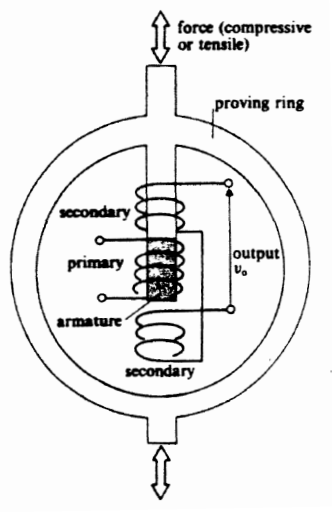
\includegraphics[width = 0.3\textwidth]{../img/Mdiagram22.png}
\end{figure}
The other forms of force transducers:
\begin{enumerate}
  \item Using the force-balance principle
  \item Using the piezoelectric effect
\end{enumerate}
\subsection{Elastic Sensing Elements}
Elastic sensing elements:
\begin{itemize}
  \item Are primary transducer (force $\rightarrow$ displacement)
  \item The force-displacement relationship should be definitive (mostly linear) 
\end{itemize}
The deformation is then detected by either measuring the strain in the member using strain gauges or measuring the displacement of a point on the elastic member.
\begin{figure}[H]
  \centering
  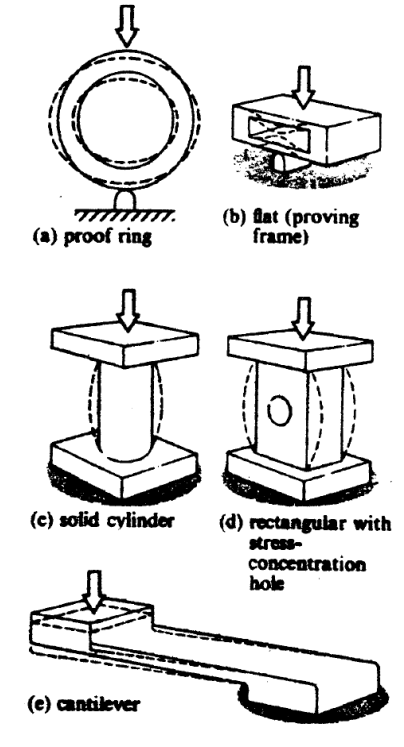
\includegraphics[width = 0.45\textwidth]{../img/Mdiagram23.png}
  \caption{Common elastic sensing elements}
\end{figure}
\textbf{Real World Example: Electronic Scale}
\begin{figure}[H]
  \centering
  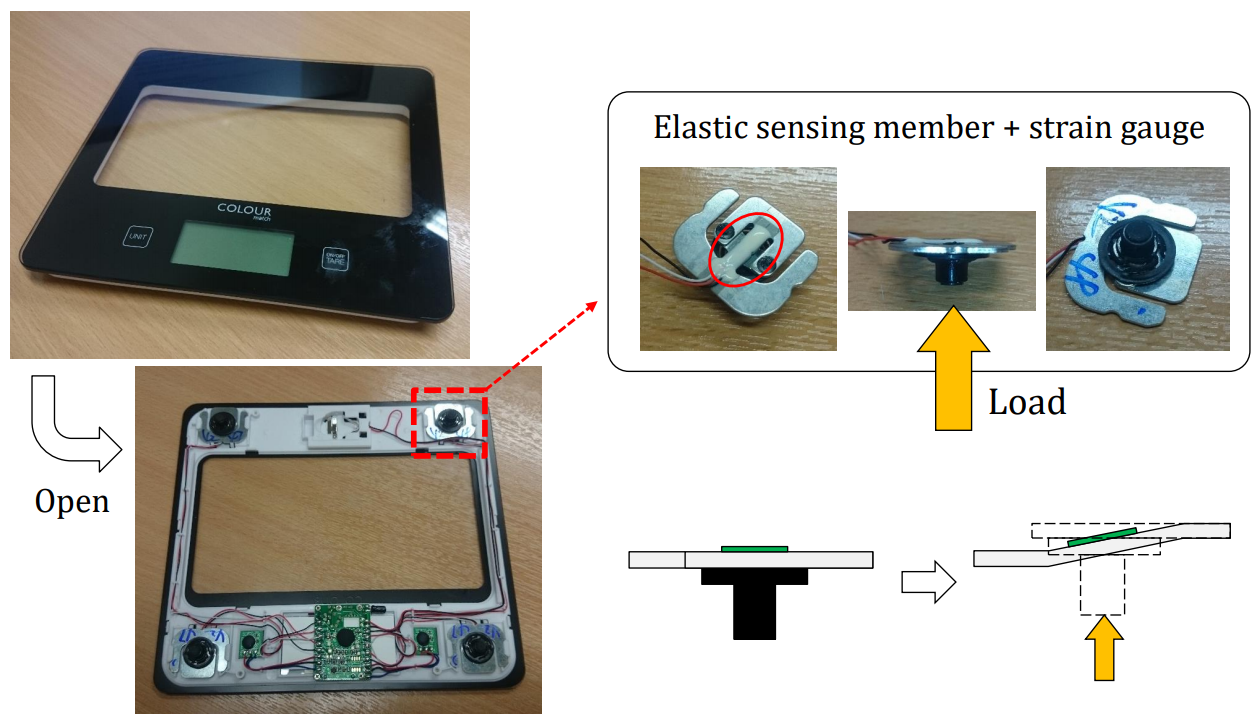
\includegraphics[width = 0.6\textwidth]{../img/Mdiagram24.png}
  \caption{Electronic Kitchen Scale}
\end{figure} 
Each transducer has a sensing member and a strain gauge. When a load is applied on the elastic member, it undergoes a displacement, which is sensed by the strain gauge. The output signal from all the transducers is used to determine a digital reading. 
\subsection{Strain Gauge Load Cell}
The most common type of load sensing cell.
\begin{figure}[H]
  \centering
  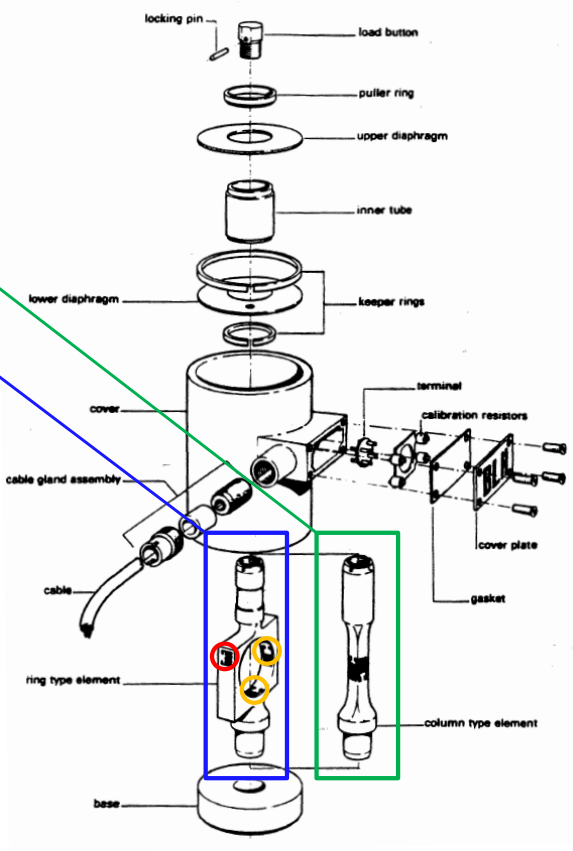
\includegraphics[width = 0.7\textwidth]{../img/Mdiagram25.png}
\end{figure}
Sensing Element Types:
\begin{itemize}
  \item Column type (green)
  \item Ring type (for smaller forces) (blue)
\end{itemize}
Each sensing element has multiple strain gauges mounted on it: typically, four measuring gauges (yellow) and two dummy gauges (red) for \textbf{span temperature compensation}.
\begin{itemize}
  \item To account for the deformation of sensing element due to temperature.
  \item To compensate “load-displacement” relationship.  
\end{itemize}
\subsection{Force Transducer Using the Force-Balance Principle}
Another type of force transducer makes use of a force balancing the input force provided by a feedback mechanism.
\begin{figure}[H]
  \centering
  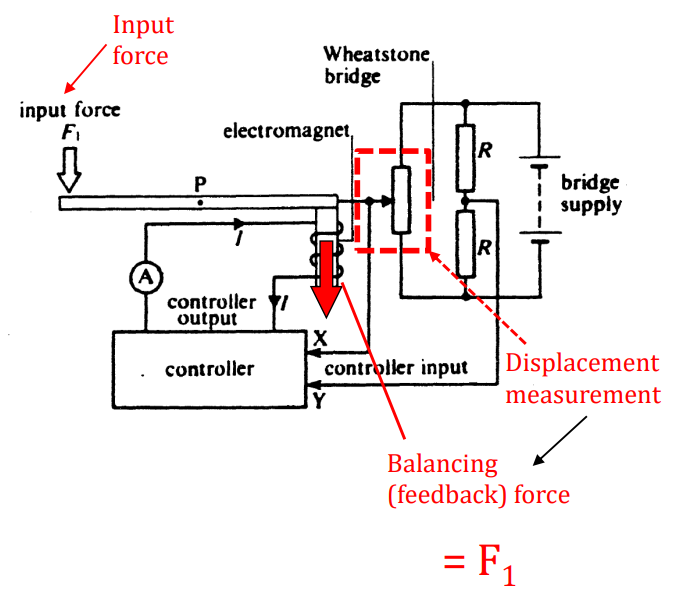
\includegraphics[width = 0.65\textwidth]{../img/Mdiagram26.png}
\end{figure}
Advantages:
\begin{enumerate}
  \item The relationship between the current I and the feedback force is linear.
  \item The rotation of the beam is almost zero all the time and the force-deflection characteristics for the beam would not be present. 
\end{enumerate}
\subsection{Piezoelectric Force Transducers}
These transducers use a piezoelectric crystal (e.g. quartz) or ceramic (e.g. PZT – lead zirconate titanate [Has to be electrically polarised before acquiring piezoelectricity]) , where electric charges of opposite polarity appear on the parallel faces of the transducer when the faces are squeezed together. \\\\
The amount of charge depends linearly on the force applied, within a limited range, and its polarity depends on the directions of the crystallographic axes.
\begin{figure}[H]
  \centering
  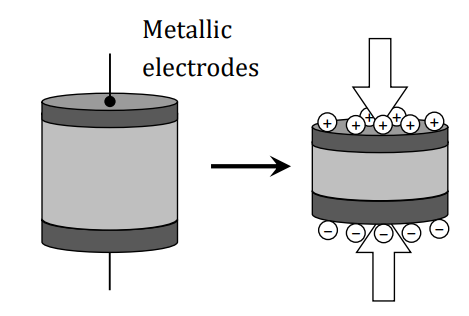
\includegraphics[width = 0.55\textwidth]{../img/Mdiagram27.png}
\end{figure}
As a whole, this works as a capacitor as well. Step input force yields charge $Q_o$, and corresponding output voltage is $V_o = Q_o/C$. \\\\
If the force is held steady, no more charge is generated but the voltage across the transducer decreases because the charges are taken by the measuring circuit as a current (i.e. flow of charge).
\begin{figure}[H]
  \centering
  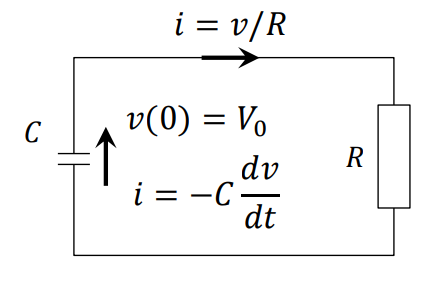
\includegraphics[width = 0.5\textwidth]{../img/Mdiagram28.png}
\end{figure}
From the current equations:
\begin{gather}
  \frac{v}{R} = -C\frac{\dif v}{\dif t}
\end{gather}
After rearranging:
\begin{gather}
  \frac{1}{v}\dif v = -\frac{1}{RC}\dif t
\end{gather}
Integration of the equation gives: 
\begin{gather}
  v=V_0e^{-\frac{t}{RC}} \longrightarrow \text{Exponential decay}
\end{gather}
Piezo\textbf{electric} transducers are \textbf{not suitable} for static or quasi-static force but are used for measuring rapidly changing forces, such as those in mechanical vibrations. (Note: Piezo\textbf{resistive} transducers are used for static measurements)
\section{Measuring Acceleration}
Acceleration transducers are called accelerometer. \\\\
A measure $g$ is widely used, indicating the acceleration experienced by a freely falling body due to gravity $(\approx 9.81 m/s^2)$. \\\\
This is a convenient standard for the calibration and in many transducers specifications, the acceleration is stated as multiples of $g$. \\\\
Several different types of accelerometers (all of them are making use of seismic-mass):
\begin{itemize}
  \item Seismic-mass accelerometer
  \item Strain-gauge accelerometer
  \item Potentiometric accelerometer
  \item Servo accelerometer
\end{itemize}
\subsection{Seismic-Mass Accelerometer}
A known mass, called seismic mass (or proof mass), is connected to some form of spring.
\begin{figure}[H]
  \centering
  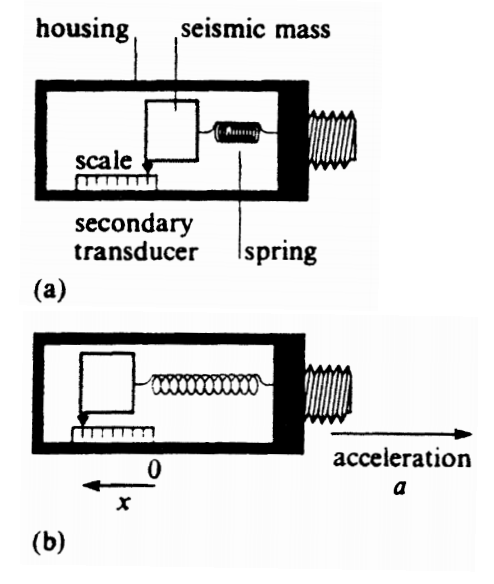
\includegraphics[width = 0.4\textwidth]{../img/Mdiagram29.png}
\end{figure}
Ignoring friction, the seismic mass displacement along the sensing axis of the accelerometer is related to the force exerted by the spring as $F = kx$ \\
($k$ is the spring constant in $N/m$). \\\\
Considering also the acceleration force $F = ma$, we get:
\begin{gather}
  ma = kx \\
  a = \frac{kx}{m}
\end{gather}
However, this only applies to \textbf{static response} of accelerometer. \\\\
\textbf{Question:} What is the expected motion of the seismic mass when the accelerometer is turned upright (measuring rapidly changing / dynamic acceleration)? (assuming the motion is limited in the sensing axis)
\begin{figure}[H]
  \centering
  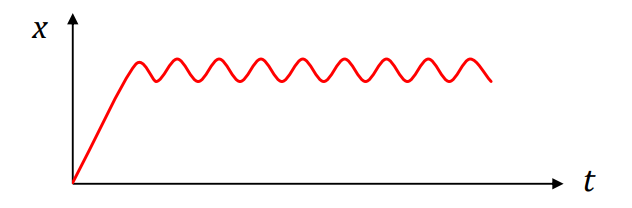
\includegraphics[width = 0.7\textwidth]{../img/Mdiagram30.png}
\end{figure}
In order to obtain a more acceptable dynamic response, a controlled amount of extra damping is added via an oil-filled dashpot.
\begin{figure}[H]
  \centering
  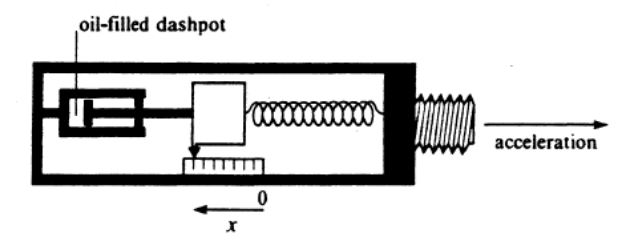
\includegraphics[width = 0.5\textwidth]{../img/Mdiagram31.png}
\end{figure}
As the result, the position of the seismic mass $x$ varies in time as shown in the figure below, in three different modes: 
\begin{itemize}
  \item Underdamped (Red)
  \item Overdamped (Green)
  \item Optimal (Blue)
\end{itemize}
where the steady state is reached relatively rapidly.
\begin{figure}[H]
  \centering
  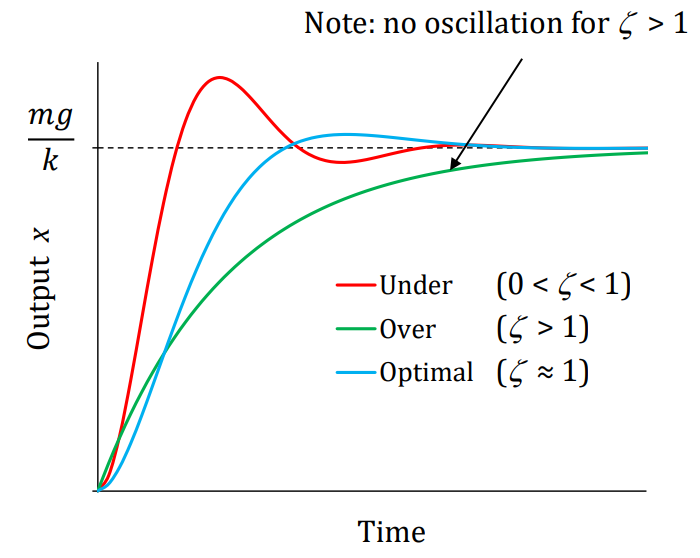
\includegraphics[width = 0.7\textwidth]{../img/Mdiagram32.png}
\end{figure}
The amount of damping in a system of this sort is expressed by means of a damping factor $\zeta$ (zeta). Without damping, the system would oscillate at its natural frequency:
\begin{gather}
  f_n = \frac{1}{2\pi}\sqrt{\frac{k}{m}}
\end{gather}
As the damping increase, the oscillating frequency changes as:
\begin{gather}
  f = f_n\sqrt{1-\zeta^2}
\end{gather}
\subsection{Strain Gauge Accelerometer}
\begin{itemize}
  \item The seismic mass is suspended from the housing by a pair of leaf springs.
  \item The closed housing contains silicon fluid for the damping.
  \item Four unbonded strain gauges are used (that is, no backing material).
\end{itemize}
\begin{figure}[H]
  \centering
  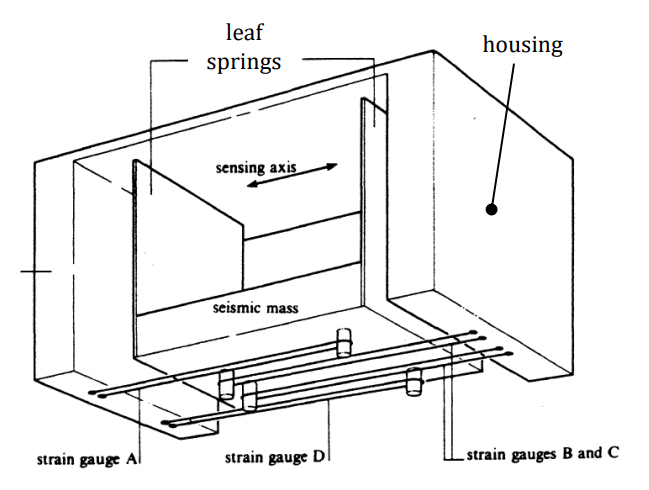
\includegraphics[width = 0.6\textwidth]{../img/Mdiagram33.png}
\end{figure}
For this type of accelerometers, the seismic mass can move in any direction, so an estimate for \textbf{cross-axis sensitivity} is important. \\
$\rightarrow$ Sensitivity to the motion in the direction normal to the sensing axis. \\
$\rightarrow$ Often mentioned in specifications, expressed in percentage of the full-scale output.
\begin{figure}[H]
  \centering
  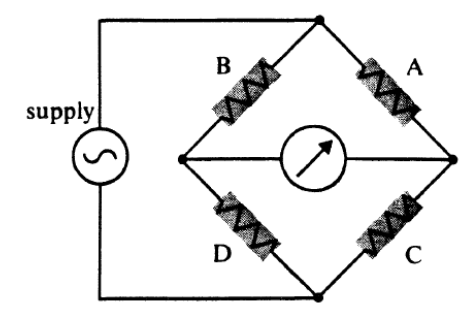
\includegraphics[width = 0.5\textwidth]{../img/Mdiagram34.png}
\end{figure}
\subsection{Potentiometric Accelerometer}
This is again a type of seismic accelerometer, has been designed for use in the flight recorder of an aircraft. It measures the vertical accelerations.
\begin{figure}[H]
  \centering
  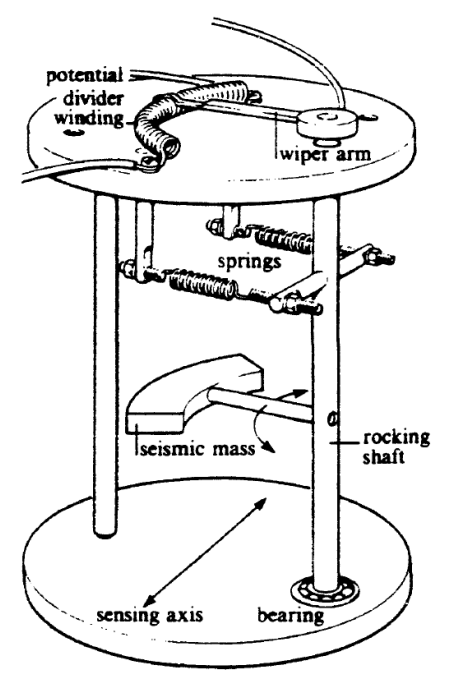
\includegraphics[width = 0.4\textwidth]{../img/Mdiagram35.png}
\end{figure}
A large cross-axis sensitivity is expected and is a problem. $\longrightarrow$ Can be avoided by a mechanism with a second shaft as shown below.
\begin{figure}[H]
  \centering
  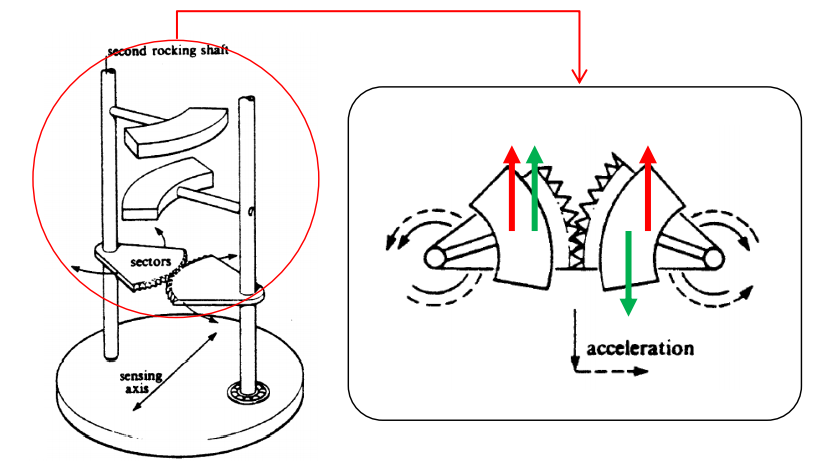
\includegraphics[width = 0.7\textwidth]{../img/Mdiagram36.png}
\end{figure}
\subsection{Servo Accelerometer}
The spring force of the previously introduced accelerometers is replaced here by an electromechanical force provided by what is called a \textbf{forcer}. \\\\
The system is similar to the force transducer using force-balance principle; the deflection of the sensing element (the beam) is detected by the light source and photodiodes (on the left) whose output is fed back to the current through the forcer coil to maintain zero deflection position via the electromechanical force generated between the coil and permanent magnet.
\begin{figure}[H]
  \centering
  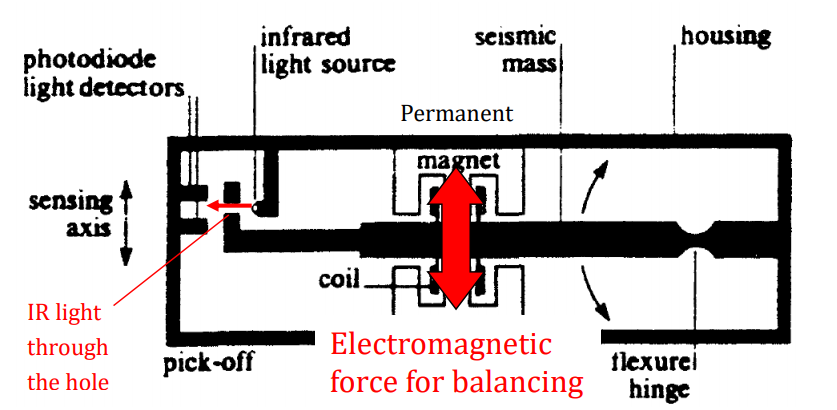
\includegraphics[width = 0.7\textwidth]{../img/Mdiagram37.png}
\end{figure}
\subsection{Piezoelectric Accelerometer}
\subsubsection{Piezoelectric effect}
\begin{itemize}
  \item Electric charge appearing on the surface of certain solid materials in response to mechanical stress applied
\end{itemize}
\begin{figure}[H]
  \centering
  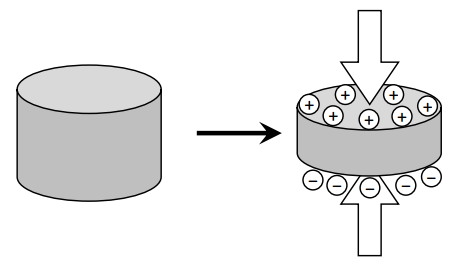
\includegraphics[width = 0.45\textwidth]{../img/Mdiagram38.png}
\end{figure}
\subsubsection{Use as accelerometer with a mass on top}
\begin{figure}[H]
  \centering
  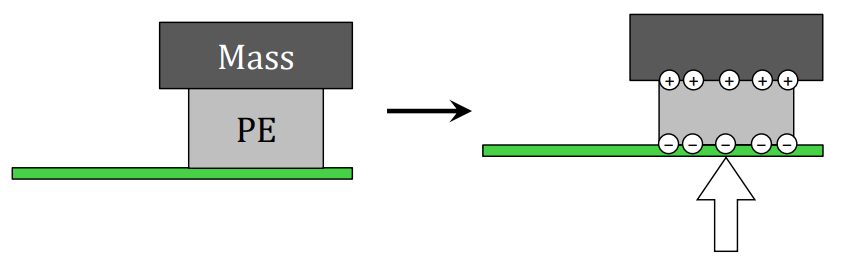
\includegraphics[width = 0.8\textwidth]{../img/Mdiagram39.png}
\end{figure}
Advantages:
\begin{itemize}
  \item Small, simple and cheap
  \item Durable (little degradation in time)
\end{itemize}
Disadvantages:
\begin{itemize}
  \item Mass of the measurement system may alter the dynamic characteristics of whole system
  \item Difficult to measure static variables
\end{itemize}
\subsection{MEMS Accelerometer}
In many nowadays applications such as mobile phones, same principles as we learned are used but in a smaller scale, in MEMS (micro-electromechanical system).
\begin{figure}[H]
  \centering
  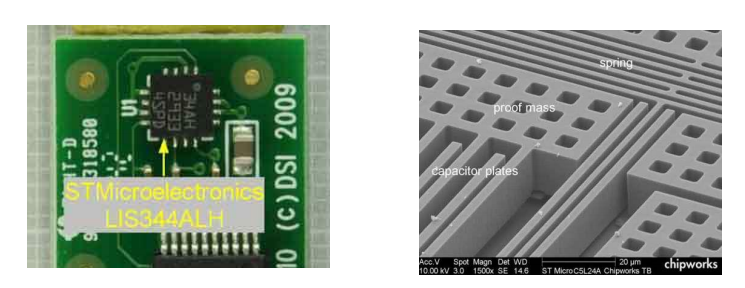
\includegraphics[width = 0.5\textwidth]{../img/Mdiagram40.png}
\end{figure}
A simplified example of MEMS accelerometer is shown below – this design is making use of a seismic mass and capacitance displacement transducer.
\begin{figure}[H]
  \centering
  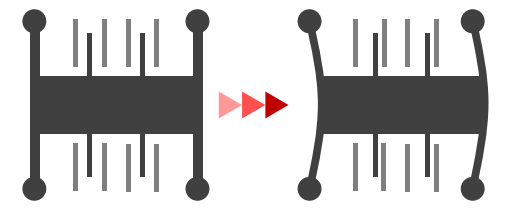
\includegraphics[width = 0.6\textwidth]{../img/Mdiagram41.png}
\end{figure}
Damping is provided by \textbf{squeeze film damping}.
\begin{figure}[H]
  \centering
  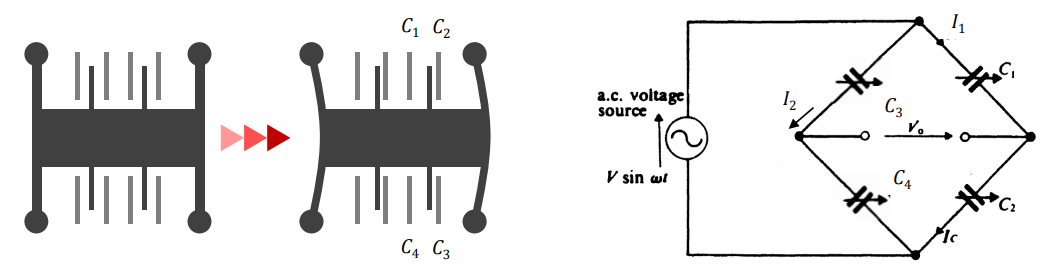
\includegraphics[width = 1\textwidth]{../img/Mdiagram42.png}
\end{figure}
Following the same derivation as in the displacement measurement:
\begin{gather}
  V_{c1} = \frac{I_1}{\omega C_1} \\
  V_{c2} = \frac{I_1}{\omega C_2} \\
  V_{c3} = \frac{I_2}{\omega C_3} \\
  V_{c4} = \frac{I_2}{\omega C_4}
\end{gather}
The voltage across $C_2$ as a fraction of the bridge energising voltage, $V$ is:
\begin{gather}
  \frac{V_{c2}}{V} = \frac{V_{c2}}{V_{c1}+V_{c2}} = \frac{\frac{I_C}{\omega C_2}}{\frac{I_C}{\omega C_1}+\frac{I_C}{\omega C_2}} = \frac{C_1}{C_1+C_2} \\[10pt]
  \frac{V_{c4}}{V} = \frac{C_3}{C_3+C_4}
\end{gather}
The capacitance in balance: 
\begin{gather}
  C_0 = \frac{\epsilon_0 A}{d}
\end{gather}
where $d$ is the balance separation. This varies with displacement as:
\begin{gather}
  C_1 = \frac{\epsilon_0 A}{d+\delta} = C_0\frac{d}{d+\delta} \\
  C_2 = C_0\frac{d}{d-\delta} \\
  C_3 = C_0\frac{d}{d-\delta} \\
  C_4 = C_0\frac{d}{d+\delta}
\end{gather}
Substituting these for the equation of the voltage across $C_2$ and $C_4$ yields:
\begin{gather}
  \frac{V_{c2}}{V} = \frac{d-\delta}{(d-\delta)+(d+\delta)} = \frac{d-\delta}{2d} \\[10pt]
  \frac{V_{c4}}{V} = \frac{d+\delta}{2d}
\end{gather}
The amplitude of the output voltage is thus:
\begin{gather}
  V_o = V_{c4}-V_{c2} = \left(\frac{d+\delta}{2d}-\frac{d-\delta}{2d}\right)V = \frac{\delta V}{d}
\end{gather}
Acceleration can then be calculated from (ignoring damping): 
\begin{gather}
  F = ma = kx \\
  a = \frac{k\delta}{m} = \frac{kdV_o}{mV}
\end{gather}


\end{document}